\documentclass[1p]{elsarticle_modified}
%\bibliographystyle{elsarticle-num}

%\usepackage[colorlinks]{hyperref}
%\usepackage{abbrmath_seonhwa} %\Abb, \Ascr, \Acal ,\Abf, \Afrak
\usepackage{amsfonts}
\usepackage{amssymb}
\usepackage{amsmath}
\usepackage{amsthm}
\usepackage{scalefnt}
\usepackage{amsbsy}
\usepackage{kotex}
\usepackage{caption}
\usepackage{subfig}
\usepackage{color}
\usepackage{graphicx}
\usepackage{xcolor} %% white, black, red, green, blue, cyan, magenta, yellow
\usepackage{float}
\usepackage{setspace}
\usepackage{hyperref}

\usepackage{tikz}
\usetikzlibrary{arrows}

\usepackage{multirow}
\usepackage{array} % fixed length table
\usepackage{hhline}

%%%%%%%%%%%%%%%%%%%%%
\makeatletter
\renewcommand*\env@matrix[1][\arraystretch]{%
	\edef\arraystretch{#1}%
	\hskip -\arraycolsep
	\let\@ifnextchar\new@ifnextchar
	\array{*\c@MaxMatrixCols c}}
\makeatother %https://tex.stackexchange.com/questions/14071/how-can-i-increase-the-line-spacing-in-a-matrix
%%%%%%%%%%%%%%%

\usepackage[normalem]{ulem}

\newcommand{\msout}[1]{\ifmmode\text{\sout{\ensuremath{#1}}}\else\sout{#1}\fi}
%SOURCE: \msout is \stkout macro in https://tex.stackexchange.com/questions/20609/strikeout-in-math-mode

\newcommand{\cancel}[1]{
	\ifmmode
	{\color{red}\msout{#1}}
	\else
	{\color{red}\sout{#1}}
	\fi
}

\newcommand{\add}[1]{
	{\color{blue}\uwave{#1}}
}

\newcommand{\replace}[2]{
	\ifmmode
	{\color{red}\msout{#1}}{\color{blue}\uwave{#2}}
	\else
	{\color{red}\sout{#1}}{\color{blue}\uwave{#2}}
	\fi
}

\newcommand{\Sol}{\mathcal{S}} %segment
\newcommand{\D}{D} %diagram
\newcommand{\A}{\mathcal{A}} %arc


%%%%%%%%%%%%%%%%%%%%%%%%%%%%%5 test

\def\sl{\operatorname{\textup{SL}}(2,\Cbb)}
\def\psl{\operatorname{\textup{PSL}}(2,\Cbb)}
\def\quan{\mkern 1mu \triangleright \mkern 1mu}

\theoremstyle{definition}
\newtheorem{thm}{Theorem}[section]
\newtheorem{prop}[thm]{Proposition}
\newtheorem{lem}[thm]{Lemma}
\newtheorem{ques}[thm]{Question}
\newtheorem{cor}[thm]{Corollary}
\newtheorem{defn}[thm]{Definition}
\newtheorem{exam}[thm]{Example}
\newtheorem{rmk}[thm]{Remark}
\newtheorem{alg}[thm]{Algorithm}

\newcommand{\I}{\sqrt{-1}}
\begin{document}

%\begin{frontmatter}
%
%\title{Boundary parabolic representations of knots up to 8 crossings}
%
%%% Group authors per affiliation:
%\author{Yunhi Cho} 
%\address{Department of Mathematics, University of Seoul, Seoul, Korea}
%\ead{yhcho@uos.ac.kr}
%
%
%\author{Seonhwa Kim} %\fnref{s_kim}}
%\address{Center for Geometry and Physics, Institute for Basic Science, Pohang, 37673, Korea}
%\ead{ryeona17@ibs.re.kr}
%
%\author{Hyuk Kim}
%\address{Department of Mathematical Sciences, Seoul National University, Seoul 08826, Korea}
%\ead{hyukkim@snu.ac.kr}
%
%\author{Seokbeom Yoon}
%\address{Department of Mathematical Sciences, Seoul National University, Seoul, 08826,  Korea}
%\ead{sbyoon15@snu.ac.kr}
%
%\begin{abstract}
%We find all boundary parabolic representation of knots up to 8 crossings.
%
%\end{abstract}
%\begin{keyword}
%    \MSC[2010] 57M25 
%\end{keyword}
%
%\end{frontmatter}

%\linenumbers
%\tableofcontents
%
\newcommand\colored[1]{\textcolor{white}{\rule[-0.35ex]{0.8em}{1.4ex}}\kern-0.8em\color{red} #1}%
%\newcommand\colored[1]{\textcolor{white}{ #1}\kern-2.17ex	\textcolor{white}{ #1}\kern-1.81ex	\textcolor{white}{ #1}\kern-2.15ex\color{red}#1	}

{\Large $\underline{12a_{0725}~(K12a_{0725})}$}

\setlength{\tabcolsep}{10pt}
\renewcommand{\arraystretch}{1.6}
\vspace{1cm}\begin{tabular}{m{100pt}>{\centering\arraybackslash}m{274pt}}
\multirow{5}{120pt}{
	\centering
	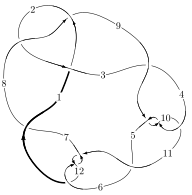
\includegraphics[width=112pt]{../../../GIT/diagram.site/Diagrams/png/1526_12a_0725.png}\\
\ \ \ A knot diagram\footnotemark}&
\allowdisplaybreaks
\textbf{Linearized knot diagam} \\
\cline{2-2}
 &
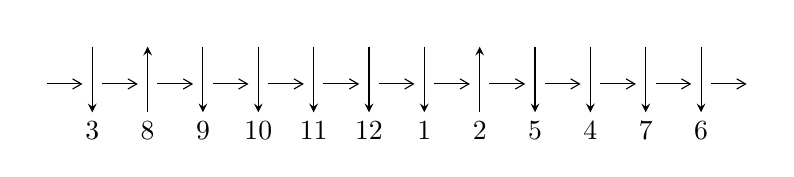
\begin{tikzpicture}[x=20pt, y=17pt]
	% nodes
	\node (C0) at (0, 0) {};
	\node (C1) at (1, 0) {};
	\node (C1U) at (1, +1) {};
	\node (C1D) at (1, -1) {3};

	\node (C2) at (2, 0) {};
	\node (C2U) at (2, +1) {};
	\node (C2D) at (2, -1) {8};

	\node (C3) at (3, 0) {};
	\node (C3U) at (3, +1) {};
	\node (C3D) at (3, -1) {9};

	\node (C4) at (4, 0) {};
	\node (C4U) at (4, +1) {};
	\node (C4D) at (4, -1) {10};

	\node (C5) at (5, 0) {};
	\node (C5U) at (5, +1) {};
	\node (C5D) at (5, -1) {11};

	\node (C6) at (6, 0) {};
	\node (C6U) at (6, +1) {};
	\node (C6D) at (6, -1) {12};

	\node (C7) at (7, 0) {};
	\node (C7U) at (7, +1) {};
	\node (C7D) at (7, -1) {1};

	\node (C8) at (8, 0) {};
	\node (C8U) at (8, +1) {};
	\node (C8D) at (8, -1) {2};

	\node (C9) at (9, 0) {};
	\node (C9U) at (9, +1) {};
	\node (C9D) at (9, -1) {5};

	\node (C10) at (10, 0) {};
	\node (C10U) at (10, +1) {};
	\node (C10D) at (10, -1) {4};

	\node (C11) at (11, 0) {};
	\node (C11U) at (11, +1) {};
	\node (C11D) at (11, -1) {7};

	\node (C12) at (12, 0) {};
	\node (C12U) at (12, +1) {};
	\node (C12D) at (12, -1) {6};
	\node (C13) at (13, 0) {};

	% arrows
	\draw[->,>={angle 60}]
	(C0) edge (C1) (C1) edge (C2) (C2) edge (C3) (C3) edge (C4) (C4) edge (C5) (C5) edge (C6) (C6) edge (C7) (C7) edge (C8) (C8) edge (C9) (C9) edge (C10) (C10) edge (C11) (C11) edge (C12) (C12) edge (C13) ;	\draw[->,>=stealth]
	(C1U) edge (C1D) (C2D) edge (C2U) (C3U) edge (C3D) (C4U) edge (C4D) (C5U) edge (C5D) (C6U) edge (C6D) (C7U) edge (C7D) (C8D) edge (C8U) (C9U) edge (C9D) (C10U) edge (C10D) (C11U) edge (C11D) (C12U) edge (C12D) ;
	\end{tikzpicture} \\
\hhline{~~} \\& 
\textbf{Solving Sequence} \\ \cline{2-2} 
 &
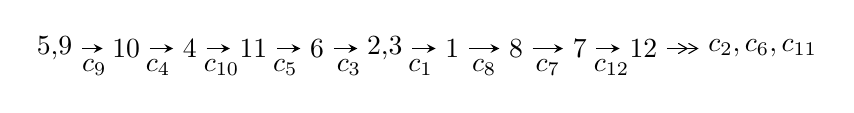
\begin{tikzpicture}[x=23pt, y=7pt]
	% node
	\node (A0) at (-1/8, 0) {5,9};
	\node (A1) at (1, 0) {10};
	\node (A2) at (2, 0) {4};
	\node (A3) at (3, 0) {11};
	\node (A4) at (4, 0) {6};
	\node (A5) at (81/16, 0) {2,3};
	\node (A6) at (49/8, 0) {1};
	\node (A7) at (57/8, 0) {8};
	\node (A8) at (65/8, 0) {7};
	\node (A9) at (73/8, 0) {12};
	\node (C1) at (1/2, -1) {$c_{9}$};
	\node (C2) at (3/2, -1) {$c_{4}$};
	\node (C3) at (5/2, -1) {$c_{10}$};
	\node (C4) at (7/2, -1) {$c_{5}$};
	\node (C5) at (9/2, -1) {$c_{3}$};
	\node (C6) at (45/8, -1) {$c_{1}$};
	\node (C7) at (53/8, -1) {$c_{8}$};
	\node (C8) at (61/8, -1) {$c_{7}$};
	\node (C9) at (69/8, -1) {$c_{12}$};
	\node (A10) at (11, 0) {$c_{2},c_{6},c_{11}$};

	% edge
	\draw[->,>=stealth]	
	(A0) edge (A1) (A1) edge (A2) (A2) edge (A3) (A3) edge (A4) (A4) edge (A5) (A5) edge (A6) (A6) edge (A7) (A7) edge (A8) (A8) edge (A9) ;
	\draw[->>,>={angle 60}]	
	(A9) edge (A10);
\end{tikzpicture} \\ 

\end{tabular} \\

\footnotetext{
The image of knot diagram is generated by the software ``\textbf{Draw programme}" developed by Andrew Bartholomew(\url{http://www.layer8.co.uk/maths/draw/index.htm\#Running-draw}), where we modified some parts for our purpose(\url{https://github.com/CATsTAILs/LinksPainter}).
}\phantom \\ \newline 
\centering \textbf{Ideals for irreducible components\footnotemark of $X_{\text{par}}$} 
 
\begin{align*}
I^u_{1}&=\langle 
- u^{15}-8 u^{13}+2 u^{12}-26 u^{11}+12 u^{10}-41 u^9+28 u^8-26 u^7+28 u^6+5 u^5+6 u^4+8 u^3-5 u^2+2 b-3 u+1,\\
\phantom{I^u_{1}}&\phantom{= \langle  }- u^{15}-8 u^{13}-26 u^{11}+2 u^{10}-41 u^9+10 u^8-26 u^7+20 u^6+5 u^5+18 u^4+8 u^3+5 u^2+2 a-3 u-1,\\
\phantom{I^u_{1}}&\phantom{= \langle  }u^{16}- u^{15}+\cdots-2 u+1\rangle \\
I^u_{2}&=\langle 
- u^{11}-4 u^9- u^8-5 u^7-3 u^6- u^5-2 u^4+u^3+b-1,\\
\phantom{I^u_{2}}&\phantom{= \langle  }- u^{13}+2 u^{12}-5 u^{11}+6 u^{10}-9 u^9+4 u^8-6 u^7-6 u^6-8 u^4+u^3-2 u^2+2 a- u-1,\\
\phantom{I^u_{2}}&\phantom{= \langle  }u^{14}+5 u^{12}+2 u^{11}+9 u^{10}+8 u^9+6 u^8+10 u^7+2 u^5- u^4-2 u^3+u^2+u+2\rangle \\
I^u_{3}&=\langle 
b- u,\;a- u,\;u^{12}- u^{11}+4 u^{10}-4 u^9+7 u^8-7 u^7+5 u^6-5 u^5+u^4- u^3+1\rangle \\
I^u_{4}&=\langle 
8 u^5 a+22 u^4 a+37 u^5+14 u^3 a+29 u^4-8 u^2 a+89 u^3+2 a u+60 u^2+97 b-37 a+82 u+35,\\
\phantom{I^u_{4}}&\phantom{= \langle  }u^5-2 u^3 a+4 u^4-2 u^2 a+6 u^3+a^2-3 a u+10 u^2-2 a+6 u+7,\;u^6+u^5+3 u^4+2 u^3+2 u^2+u-1\rangle \\
I^u_{5}&=\langle 
b- u,\;a- u,\;u^6+u^5+3 u^4+2 u^3+2 u^2+u-1\rangle \\
I^u_{6}&=\langle 
b- u,\;a- u+1,\;u^2+1\rangle \\
\\
\end{align*}
\raggedright * 6 irreducible components of $\dim_{\mathbb{C}}=0$, with total 62 representations.\\
\footnotetext{All coefficients of polynomials are rational numbers. But the coefficients are sometimes approximated in decimal forms when there is not enough margin.}
\newpage
\renewcommand{\arraystretch}{1}
\centering \section*{I. $I^u_{1}= \langle - u^{15}-8 u^{13}+\cdots+2 b+1,\;- u^{15}-8 u^{13}+\cdots+2 a-1,\;u^{16}- u^{15}+\cdots-2 u+1 \rangle$}
\flushleft \textbf{(i) Arc colorings}\\
\begin{tabular}{m{7pt} m{180pt} m{7pt} m{180pt} }
\flushright $a_{5}=$&$\begin{pmatrix}0\\u\end{pmatrix}$ \\
\flushright $a_{9}=$&$\begin{pmatrix}1\\0\end{pmatrix}$ \\
\flushright $a_{10}=$&$\begin{pmatrix}1\\u^2\end{pmatrix}$ \\
\flushright $a_{4}=$&$\begin{pmatrix}u\\u^3+u\end{pmatrix}$ \\
\flushright $a_{11}=$&$\begin{pmatrix}u^2+1\\u^4+2 u^2\end{pmatrix}$ \\
\flushright $a_{6}=$&$\begin{pmatrix}- u^5-2 u^3- u\\- u^7-3 u^5-2 u^3+u\end{pmatrix}$ \\
\flushright $a_{2}=$&$\begin{pmatrix}\frac{1}{2} u^{15}+4 u^{13}+\cdots+\frac{3}{2} u+\frac{1}{2}\\\frac{1}{2} u^{15}+4 u^{13}+\cdots+\frac{3}{2} u-\frac{1}{2}\end{pmatrix}$ \\
\flushright $a_{3}=$&$\begin{pmatrix}u^3+2 u\\u^3+u\end{pmatrix}$ \\
\flushright $a_{1}=$&$\begin{pmatrix}- u^6-3 u^4-2 u^2+1\\\frac{1}{2} u^{15}- u^{14}+\cdots+\frac{3}{2} u-\frac{1}{2}\end{pmatrix}$ \\
\flushright $a_{8}=$&$\begin{pmatrix}- u^9-4 u^7-5 u^5+3 u\\-\frac{1}{2} u^{15}-3 u^{13}+\cdots-\frac{1}{2} u-\frac{1}{2}\end{pmatrix}$ \\
\flushright $a_{7}=$&$\begin{pmatrix}u^3+2 u\\-\frac{1}{2} u^{15}-3 u^{13}+\cdots-\frac{1}{2} u-\frac{1}{2}\end{pmatrix}$ \\
\flushright $a_{12}=$&$\begin{pmatrix}- u^4- u^2+1\\\frac{1}{2} u^{15}- u^{14}+\cdots+\frac{3}{2} u-\frac{1}{2}\end{pmatrix}$\\&\end{tabular}
\flushleft \textbf{(ii) Obstruction class $= -1$}\\~\\
\flushleft \textbf{(iii) Cusp Shapes $= 4 u^{15}-4 u^{14}+30 u^{13}-28 u^{12}+90 u^{11}-76 u^{10}+122 u^9-88 u^8+40 u^7-16 u^6-64 u^5+36 u^4-34 u^3+22 u-16$}\\~\\
\newpage\renewcommand{\arraystretch}{1}
\flushleft \textbf{(iv) u-Polynomials at the component}\newline \\
\begin{tabular}{m{50pt}|m{274pt}}
Crossings & \hspace{64pt}u-Polynomials at each crossing \\
\hline $$\begin{aligned}c_{1}\end{aligned}$$&$\begin{aligned}
&u^{16}+8 u^{15}+\cdots+11 u+4
\end{aligned}$\\
\hline $$\begin{aligned}c_{2},c_{8}\end{aligned}$$&$\begin{aligned}
&u^{16}-2 u^{15}+\cdots-3 u+2
\end{aligned}$\\
\hline $$\begin{aligned}c_{3},c_{5},c_{7}\end{aligned}$$&$\begin{aligned}
&u^{16}+2 u^{15}+\cdots+12 u+8
\end{aligned}$\\
\hline $$\begin{aligned}c_{4},c_{6},c_{9}\\c_{10},c_{11},c_{12}\end{aligned}$$&$\begin{aligned}
&u^{16}+u^{15}+\cdots+2 u+1
\end{aligned}$\\
\hline
\end{tabular}\\~\\
\newpage\renewcommand{\arraystretch}{1}
\flushleft \textbf{(v) Riley Polynomials at the component}\newline \\
\begin{tabular}{m{50pt}|m{274pt}}
Crossings & \hspace{64pt}Riley Polynomials at each crossing \\
\hline $$\begin{aligned}c_{1}\end{aligned}$$&$\begin{aligned}
&y^{16}+24 y^{14}+\cdots-33 y+16
\end{aligned}$\\
\hline $$\begin{aligned}c_{2},c_{8}\end{aligned}$$&$\begin{aligned}
&y^{16}+8 y^{15}+\cdots+11 y+4
\end{aligned}$\\
\hline $$\begin{aligned}c_{3},c_{5},c_{7}\end{aligned}$$&$\begin{aligned}
&y^{16}-14 y^{15}+\cdots+496 y+64
\end{aligned}$\\
\hline $$\begin{aligned}c_{4},c_{6},c_{9}\\c_{10},c_{11},c_{12}\end{aligned}$$&$\begin{aligned}
&y^{16}+15 y^{15}+\cdots+4 y+1
\end{aligned}$\\
\hline
\end{tabular}\\~\\
\newpage\flushleft \textbf{(vi) Complex Volumes and Cusp Shapes}
$$\begin{array}{c|c|c}  
\text{Solutions to }I^u_{1}& \I (\text{vol} + \sqrt{-1}CS) & \text{Cusp shape}\\
 \hline 
\begin{aligned}
u &= \phantom{-}0.896754 + 0.031752 I \\
a &= \phantom{-}0.17672 + 2.61210 I \\
b &= -0.465246 + 1.250080 I\end{aligned}
 & -11.44060 - 4.76307 I & -15.3726 + 3.2989 I \\ \hline\begin{aligned}
u &= \phantom{-}0.896754 - 0.031752 I \\
a &= \phantom{-}0.17672 - 2.61210 I \\
b &= -0.465246 - 1.250080 I\end{aligned}
 & -11.44060 + 4.76307 I & -15.3726 - 3.2989 I \\ \hline\begin{aligned}
u &= -0.177081 + 1.342100 I \\
a &= -0.281404 + 0.454739 I \\
b &= \phantom{-}0.725499 - 0.391212 I\end{aligned}
 & \phantom{-}8.15821 + 4.40873 I & \phantom{-}0.01113 - 3.61674 I \\ \hline\begin{aligned}
u &= -0.177081 - 1.342100 I \\
a &= -0.281404 - 0.454739 I \\
b &= \phantom{-}0.725499 + 0.391212 I\end{aligned}
 & \phantom{-}8.15821 - 4.40873 I & \phantom{-}0.01113 + 3.61674 I \\ \hline\begin{aligned}
u &= \phantom{-}0.399274 + 1.311870 I \\
a &= -0.110245 + 0.614867 I \\
b &= -0.897959 - 0.093377 I\end{aligned}
 & \phantom{-}0.55749 - 9.14366 I & -4.61411 + 5.72614 I \\ \hline\begin{aligned}
u &= \phantom{-}0.399274 - 1.311870 I \\
a &= -0.110245 - 0.614867 I \\
b &= -0.897959 + 0.093377 I\end{aligned}
 & \phantom{-}0.55749 + 9.14366 I & -4.61411 - 5.72614 I \\ \hline\begin{aligned}
u &= -0.037558 + 1.371140 I \\
a &= \phantom{-}0.952917 + 0.035835 I \\
b &= -0.623542 - 0.745700 I\end{aligned}
 & \phantom{-}9.86121 + 2.40714 I & \phantom{-}1.11944 - 3.44004 I \\ \hline\begin{aligned}
u &= -0.037558 - 1.371140 I \\
a &= \phantom{-}0.952917 - 0.035835 I \\
b &= -0.623542 + 0.745700 I\end{aligned}
 & \phantom{-}9.86121 - 2.40714 I & \phantom{-}1.11944 + 3.44004 I \\ \hline\begin{aligned}
u &= \phantom{-}0.240518 + 1.356540 I \\
a &= -1.46246 - 0.89499 I \\
b &= \phantom{-}0.561956 - 1.036960 I\end{aligned}
 & \phantom{-}6.29728 - 9.25950 I & -3.29029 + 8.32178 I \\ \hline\begin{aligned}
u &= \phantom{-}0.240518 - 1.356540 I \\
a &= -1.46246 + 0.89499 I \\
b &= \phantom{-}0.561956 + 1.036960 I\end{aligned}
 & \phantom{-}6.29728 + 9.25950 I & -3.29029 - 8.32178 I\\
 \hline 
 \end{array}$$\newpage$$\begin{array}{c|c|c}  
\text{Solutions to }I^u_{1}& \I (\text{vol} + \sqrt{-1}CS) & \text{Cusp shape}\\
 \hline 
\begin{aligned}
u &= -0.598794 + 0.151071 I \\
a &= -0.88900 + 2.25691 I \\
b &= \phantom{-}0.359947 + 1.044940 I\end{aligned}
 & -3.27788 + 3.09462 I & -15.6158 - 6.1007 I \\ \hline\begin{aligned}
u &= -0.598794 - 0.151071 I \\
a &= -0.88900 - 2.25691 I \\
b &= \phantom{-}0.359947 - 1.044940 I\end{aligned}
 & -3.27788 - 3.09462 I & -15.6158 + 6.1007 I \\ \hline\begin{aligned}
u &= -0.420730 + 1.328670 I \\
a &= \phantom{-}1.38895 - 1.73157 I \\
b &= -0.514655 - 1.242600 I\end{aligned}
 & -2.9192 + 14.2327 I & -7.70275 - 8.58885 I \\ \hline\begin{aligned}
u &= -0.420730 - 1.328670 I \\
a &= \phantom{-}1.38895 + 1.73157 I \\
b &= -0.514655 + 1.242600 I\end{aligned}
 & -2.9192 - 14.2327 I & -7.70275 + 8.58885 I \\ \hline\begin{aligned}
u &= \phantom{-}0.197618 + 0.311751 I \\
a &= \phantom{-}1.224520 + 0.293518 I \\
b &= -0.146001 + 0.823219 I\end{aligned}
 & -0.656687 - 0.955703 I & -10.53509 + 6.55993 I \\ \hline\begin{aligned}
u &= \phantom{-}0.197618 - 0.311751 I \\
a &= \phantom{-}1.224520 - 0.293518 I \\
b &= -0.146001 - 0.823219 I\end{aligned}
 & -0.656687 + 0.955703 I & -10.53509 - 6.55993 I\\
 \hline 
 \end{array}$$\newpage\newpage\renewcommand{\arraystretch}{1}
\centering \section*{II. $I^u_{2}= \langle - u^{11}-4 u^9+\cdots+b-1,\;- u^{13}+2 u^{12}+\cdots+2 a-1,\;u^{14}+5 u^{12}+\cdots+u+2 \rangle$}
\flushleft \textbf{(i) Arc colorings}\\
\begin{tabular}{m{7pt} m{180pt} m{7pt} m{180pt} }
\flushright $a_{5}=$&$\begin{pmatrix}0\\u\end{pmatrix}$ \\
\flushright $a_{9}=$&$\begin{pmatrix}1\\0\end{pmatrix}$ \\
\flushright $a_{10}=$&$\begin{pmatrix}1\\u^2\end{pmatrix}$ \\
\flushright $a_{4}=$&$\begin{pmatrix}u\\u^3+u\end{pmatrix}$ \\
\flushright $a_{11}=$&$\begin{pmatrix}u^2+1\\u^4+2 u^2\end{pmatrix}$ \\
\flushright $a_{6}=$&$\begin{pmatrix}- u^5-2 u^3- u\\- u^7-3 u^5-2 u^3+u\end{pmatrix}$ \\
\flushright $a_{2}=$&$\begin{pmatrix}\frac{1}{2} u^{13}- u^{12}+\cdots+\frac{1}{2} u+\frac{1}{2}\\u^{11}+4 u^9+u^8+5 u^7+3 u^6+u^5+2 u^4- u^3+1\end{pmatrix}$ \\
\flushright $a_{3}=$&$\begin{pmatrix}u^3+2 u\\u^3+u\end{pmatrix}$ \\
\flushright $a_{1}=$&$\begin{pmatrix}-\frac{1}{2} u^{13}-\frac{3}{2} u^{11}+\cdots+\frac{1}{2} u+\frac{1}{2}\\u^{12}+u^{11}+4 u^{10}+4 u^9+6 u^8+5 u^7+3 u^6- u^4-2 u^3+u+1\end{pmatrix}$ \\
\flushright $a_{8}=$&$\begin{pmatrix}\frac{1}{2} u^{13}+\frac{3}{2} u^{11}+\cdots-\frac{1}{2} u-\frac{1}{2}\\- u^{12}-4 u^{10}- u^9-5 u^8-3 u^7- u^6-2 u^5+u^4- u^2- u-1\end{pmatrix}$ \\
\flushright $a_{7}=$&$\begin{pmatrix}-\frac{1}{2} u^{13}-\frac{3}{2} u^{11}+\cdots-\frac{1}{2} u+\frac{1}{2}\\u^{12}+u^{11}+4 u^{10}+4 u^9+6 u^8+5 u^7+3 u^6- u^4-2 u^3+u+1\end{pmatrix}$ \\
\flushright $a_{12}=$&$\begin{pmatrix}\frac{1}{2} u^{13}+\frac{7}{2} u^{11}+\cdots+\frac{1}{2} u+\frac{5}{2}\\u^{13}+5 u^{11}+9 u^9+5 u^7-3 u^5+2 u^4-3 u^3+4 u^2+1\end{pmatrix}$\\&\end{tabular}
\flushleft \textbf{(ii) Obstruction class $= -1$}\\~\\
\flushleft \textbf{(iii) Cusp Shapes $= 4 u^{12}-4 u^{11}+16 u^{10}-8 u^9+20 u^8+4 u^7+4 u^6+20 u^5-4 u^4+12 u^3-6$}\\~\\
\newpage\renewcommand{\arraystretch}{1}
\flushleft \textbf{(iv) u-Polynomials at the component}\newline \\
\begin{tabular}{m{50pt}|m{274pt}}
Crossings & \hspace{64pt}u-Polynomials at each crossing \\
\hline $$\begin{aligned}c_{1}\end{aligned}$$&$\begin{aligned}
&(u^7+4 u^6+8 u^5+7 u^4+2 u^3-3 u^2-2 u-1)^2
\end{aligned}$\\
\hline $$\begin{aligned}c_{2},c_{8}\end{aligned}$$&$\begin{aligned}
&(u^7+2 u^5- u^4+2 u^3- u^2-1)^2
\end{aligned}$\\
\hline $$\begin{aligned}c_{3},c_{5},c_{7}\end{aligned}$$&$\begin{aligned}
&(u^7-3 u^6+u^5+2 u^4+2 u^3-3 u^2+u-2)^2
\end{aligned}$\\
\hline $$\begin{aligned}c_{4},c_{6},c_{9}\\c_{10},c_{11},c_{12}\end{aligned}$$&$\begin{aligned}
&u^{14}+5 u^{12}+\cdots- u+2
\end{aligned}$\\
\hline
\end{tabular}\\~\\
\newpage\renewcommand{\arraystretch}{1}
\flushleft \textbf{(v) Riley Polynomials at the component}\newline \\
\begin{tabular}{m{50pt}|m{274pt}}
Crossings & \hspace{64pt}Riley Polynomials at each crossing \\
\hline $$\begin{aligned}c_{1}\end{aligned}$$&$\begin{aligned}
&(y^7+12 y^5+3 y^4+22 y^3-3 y^2-2 y-1)^2
\end{aligned}$\\
\hline $$\begin{aligned}c_{2},c_{8}\end{aligned}$$&$\begin{aligned}
&(y^7+4 y^6+8 y^5+7 y^4+2 y^3-3 y^2-2 y-1)^2
\end{aligned}$\\
\hline $$\begin{aligned}c_{3},c_{5},c_{7}\end{aligned}$$&$\begin{aligned}
&(y^7-7 y^6+17 y^5-16 y^4+6 y^3+3 y^2-11 y-4)^2
\end{aligned}$\\
\hline $$\begin{aligned}c_{4},c_{6},c_{9}\\c_{10},c_{11},c_{12}\end{aligned}$$&$\begin{aligned}
&y^{14}+10 y^{13}+\cdots+3 y+4
\end{aligned}$\\
\hline
\end{tabular}\\~\\
\newpage\flushleft \textbf{(vi) Complex Volumes and Cusp Shapes}
$$\begin{array}{c|c|c}  
\text{Solutions to }I^u_{2}& \I (\text{vol} + \sqrt{-1}CS) & \text{Cusp shape}\\
 \hline 
\begin{aligned}
u &= -0.909403 + 0.064443 I \\
a &= -0.15740 + 2.55157 I \\
b &= \phantom{-}0.489252 + 1.239920 I\end{aligned}
 & -7.27584 + 9.47458 I & -11.52754 - 6.21855 I \\ \hline\begin{aligned}
u &= -0.909403 - 0.064443 I \\
a &= -0.15740 - 2.55157 I \\
b &= \phantom{-}0.489252 - 1.239920 I\end{aligned}
 & -7.27584 - 9.47458 I & -11.52754 + 6.21855 I \\ \hline\begin{aligned}
u &= \phantom{-}0.004458 + 1.241100 I \\
a &= -1.103090 + 0.868476 I \\
b &= \phantom{-}0.391915 - 0.631080 I\end{aligned}
 & \phantom{-}3.69786 - 1.46776 I & -2.58766 + 4.85424 I \\ \hline\begin{aligned}
u &= \phantom{-}0.004458 - 1.241100 I \\
a &= -1.103090 - 0.868476 I \\
b &= \phantom{-}0.391915 + 0.631080 I\end{aligned}
 & \phantom{-}3.69786 + 1.46776 I & -2.58766 - 4.85424 I \\ \hline\begin{aligned}
u &= \phantom{-}0.689055 + 0.275978 I \\
a &= \phantom{-}0.52249 + 2.02022 I \\
b &= -0.468927 + 1.008510 I\end{aligned}
 & \phantom{-}1.13946 - 6.00484 I & -8.26608 + 8.08638 I \\ \hline\begin{aligned}
u &= \phantom{-}0.689055 - 0.275978 I \\
a &= \phantom{-}0.52249 - 2.02022 I \\
b &= -0.468927 - 1.008510 I\end{aligned}
 & \phantom{-}1.13946 + 6.00484 I & -8.26608 - 8.08638 I \\ \hline\begin{aligned}
u &= -0.396373 + 0.610024 I \\
a &= -0.351244 + 1.089890 I \\
b &= \phantom{-}0.391915 + 0.631080 I\end{aligned}
 & \phantom{-}3.69786 + 1.46776 I & -2.58766 - 4.85424 I \\ \hline\begin{aligned}
u &= -0.396373 - 0.610024 I \\
a &= -0.351244 - 1.089890 I \\
b &= \phantom{-}0.391915 - 0.631080 I\end{aligned}
 & \phantom{-}3.69786 - 1.46776 I & -2.58766 + 4.85424 I \\ \hline\begin{aligned}
u &= \phantom{-}0.412241 + 1.228750 I \\
a &= -0.088236 + 0.731499 I \\
b &= -0.824481\phantom{ +0.000000I}\end{aligned}
 & -0.0577569\phantom{ +0.000000I} & -5.23744 + 0. I\phantom{ +0.000000I} \\ \hline\begin{aligned}
u &= \phantom{-}0.412241 - 1.228750 I \\
a &= -0.088236 - 0.731499 I \\
b &= -0.824481\phantom{ +0.000000I}\end{aligned}
 & -0.0577569\phantom{ +0.000000I} & -5.23744 + 0. I\phantom{ +0.000000I}\\
 \hline 
 \end{array}$$\newpage$$\begin{array}{c|c|c}  
\text{Solutions to }I^u_{2}& \I (\text{vol} + \sqrt{-1}CS) & \text{Cusp shape}\\
 \hline 
\begin{aligned}
u &= -0.220128 + 1.284480 I \\
a &= \phantom{-}1.90275 - 0.76301 I \\
b &= -0.468927 - 1.008510 I\end{aligned}
 & \phantom{-}1.13946 + 6.00484 I & -8.26608 - 8.08638 I \\ \hline\begin{aligned}
u &= -0.220128 - 1.284480 I \\
a &= \phantom{-}1.90275 + 0.76301 I \\
b &= -0.468927 + 1.008510 I\end{aligned}
 & \phantom{-}1.13946 - 6.00484 I & -8.26608 + 8.08638 I \\ \hline\begin{aligned}
u &= \phantom{-}0.420151 + 1.304360 I \\
a &= -1.47527 - 1.77944 I \\
b &= \phantom{-}0.489252 - 1.239920 I\end{aligned}
 & -7.27584 - 9.47458 I & -11.52754 + 6.21855 I \\ \hline\begin{aligned}
u &= \phantom{-}0.420151 - 1.304360 I \\
a &= -1.47527 + 1.77944 I \\
b &= \phantom{-}0.489252 + 1.239920 I\end{aligned}
 & -7.27584 + 9.47458 I & -11.52754 - 6.21855 I\\
 \hline 
 \end{array}$$\newpage\newpage\renewcommand{\arraystretch}{1}
\centering \section*{III. $I^u_{3}= \langle b- u,\;a- u,\;u^{12}- u^{11}+\cdots- u^3+1 \rangle$}
\flushleft \textbf{(i) Arc colorings}\\
\begin{tabular}{m{7pt} m{180pt} m{7pt} m{180pt} }
\flushright $a_{5}=$&$\begin{pmatrix}0\\u\end{pmatrix}$ \\
\flushright $a_{9}=$&$\begin{pmatrix}1\\0\end{pmatrix}$ \\
\flushright $a_{10}=$&$\begin{pmatrix}1\\u^2\end{pmatrix}$ \\
\flushright $a_{4}=$&$\begin{pmatrix}u\\u^3+u\end{pmatrix}$ \\
\flushright $a_{11}=$&$\begin{pmatrix}u^2+1\\u^4+2 u^2\end{pmatrix}$ \\
\flushright $a_{6}=$&$\begin{pmatrix}- u^5-2 u^3- u\\- u^7-3 u^5-2 u^3+u\end{pmatrix}$ \\
\flushright $a_{2}=$&$\begin{pmatrix}u\\u\end{pmatrix}$ \\
\flushright $a_{3}=$&$\begin{pmatrix}u^3+2 u\\u^3+u\end{pmatrix}$ \\
\flushright $a_{1}=$&$\begin{pmatrix}u^5+2 u^3+u\\u^5+u^3+u\end{pmatrix}$ \\
\flushright $a_{8}=$&$\begin{pmatrix}u^2+1\\u^2\end{pmatrix}$ \\
\flushright $a_{7}=$&$\begin{pmatrix}- u^8-3 u^6-3 u^4+1\\- u^8-2 u^6-2 u^4\end{pmatrix}$ \\
\flushright $a_{12}=$&$\begin{pmatrix}-2 u^{11}-8 u^9-13 u^7-6 u^5+u^4+4 u^3+3 u^2+4 u+3\\-2 u^{11}-8 u^9-13 u^7+u^6-7 u^5+4 u^4+2 u^3+5 u^2+3 u+2\end{pmatrix}$\\&\end{tabular}
\flushleft \textbf{(ii) Obstruction class $= -1$}\\~\\
\flushleft \textbf{(iii) Cusp Shapes $= 4 u^9+12 u^7+12 u^5-4 u^3-8 u-10$}\\~\\
\newpage\renewcommand{\arraystretch}{1}
\flushleft \textbf{(iv) u-Polynomials at the component}\newline \\
\begin{tabular}{m{50pt}|m{274pt}}
Crossings & \hspace{64pt}u-Polynomials at each crossing \\
\hline $$\begin{aligned}c_{1}\end{aligned}$$&$\begin{aligned}
&u^{12}+7 u^{11}+\cdots+2 u^2+1
\end{aligned}$\\
\hline $$\begin{aligned}c_{2},c_{4},c_{8}\\c_{9},c_{10}\end{aligned}$$&$\begin{aligned}
&u^{12}+u^{11}+4 u^{10}+4 u^9+7 u^8+7 u^7+5 u^6+5 u^5+u^4+u^3+1
\end{aligned}$\\
\hline $$\begin{aligned}c_{3},c_{5},c_{7}\end{aligned}$$&$\begin{aligned}
&(u^6+u^5-3 u^4-2 u^3+2 u^2- u-1)^2
\end{aligned}$\\
\hline $$\begin{aligned}c_{6},c_{11},c_{12}\end{aligned}$$&$\begin{aligned}
&(u^6- u^5+3 u^4-2 u^3+2 u^2- u-1)^2
\end{aligned}$\\
\hline
\end{tabular}\\~\\
\newpage\renewcommand{\arraystretch}{1}
\flushleft \textbf{(v) Riley Polynomials at the component}\newline \\
\begin{tabular}{m{50pt}|m{274pt}}
Crossings & \hspace{64pt}Riley Polynomials at each crossing \\
\hline $$\begin{aligned}c_{1}\end{aligned}$$&$\begin{aligned}
&y^{12}-5 y^{11}+\cdots+4 y+1
\end{aligned}$\\
\hline $$\begin{aligned}c_{2},c_{4},c_{8}\\c_{9},c_{10}\end{aligned}$$&$\begin{aligned}
&y^{12}+7 y^{11}+\cdots+2 y^2+1
\end{aligned}$\\
\hline $$\begin{aligned}c_{3},c_{5},c_{7}\end{aligned}$$&$\begin{aligned}
&(y^6-7 y^5+17 y^4-16 y^3+6 y^2-5 y+1)^2
\end{aligned}$\\
\hline $$\begin{aligned}c_{6},c_{11},c_{12}\end{aligned}$$&$\begin{aligned}
&(y^6+5 y^5+9 y^4+4 y^3-6 y^2-5 y+1)^2
\end{aligned}$\\
\hline
\end{tabular}\\~\\
\newpage\flushleft \textbf{(vi) Complex Volumes and Cusp Shapes}
$$\begin{array}{c|c|c}  
\text{Solutions to }I^u_{3}& \I (\text{vol} + \sqrt{-1}CS) & \text{Cusp shape}\\
 \hline 
\begin{aligned}
u &= \phantom{-}0.386547 + 0.899125 I \\
a &= \phantom{-}0.386547 + 0.899125 I \\
b &= \phantom{-}0.386547 + 0.899125 I\end{aligned}
 & \phantom{-}2.96024 + 1.97241 I & -4.57572 - 3.68478 I \\ \hline\begin{aligned}
u &= \phantom{-}0.386547 - 0.899125 I \\
a &= \phantom{-}0.386547 - 0.899125 I \\
b &= \phantom{-}0.386547 - 0.899125 I\end{aligned}
 & \phantom{-}2.96024 - 1.97241 I & -4.57572 + 3.68478 I \\ \hline\begin{aligned}
u &= -0.206575 + 1.062080 I \\
a &= -0.206575 + 1.062080 I \\
b &= -0.206575 + 1.062080 I\end{aligned}
 & -0.738851\phantom{ +0.000000I} & -13.41678 + 0. I\phantom{ +0.000000I} \\ \hline\begin{aligned}
u &= -0.206575 - 1.062080 I \\
a &= -0.206575 - 1.062080 I \\
b &= -0.206575 - 1.062080 I\end{aligned}
 & -0.738851\phantom{ +0.000000I} & -13.41678 + 0. I\phantom{ +0.000000I} \\ \hline\begin{aligned}
u &= \phantom{-}0.869654 + 0.049931 I \\
a &= \phantom{-}0.869654 + 0.049931 I \\
b &= \phantom{-}0.869654 + 0.049931 I\end{aligned}
 & -3.69558 - 4.59213 I & -8.58114 + 3.20482 I \\ \hline\begin{aligned}
u &= \phantom{-}0.869654 - 0.049931 I \\
a &= \phantom{-}0.869654 - 0.049931 I \\
b &= \phantom{-}0.869654 - 0.049931 I\end{aligned}
 & -3.69558 + 4.59213 I & -8.58114 - 3.20482 I \\ \hline\begin{aligned}
u &= -0.460851 + 1.226450 I \\
a &= -0.460851 + 1.226450 I \\
b &= -0.460851 + 1.226450 I\end{aligned}
 & -3.69558 - 4.59213 I & -8.58114 + 3.20482 I \\ \hline\begin{aligned}
u &= -0.460851 - 1.226450 I \\
a &= -0.460851 - 1.226450 I \\
b &= -0.460851 - 1.226450 I\end{aligned}
 & -3.69558 + 4.59213 I & -8.58114 - 3.20482 I \\ \hline\begin{aligned}
u &= \phantom{-}0.436607 + 1.253750 I \\
a &= \phantom{-}0.436607 + 1.253750 I \\
b &= \phantom{-}0.436607 + 1.253750 I\end{aligned}
 & -7.66009\phantom{ +0.000000I} & -12.26950 + 0. I\phantom{ +0.000000I} \\ \hline\begin{aligned}
u &= \phantom{-}0.436607 - 1.253750 I \\
a &= \phantom{-}0.436607 - 1.253750 I \\
b &= \phantom{-}0.436607 - 1.253750 I\end{aligned}
 & -7.66009\phantom{ +0.000000I} & -12.26950 + 0. I\phantom{ +0.000000I}\\
 \hline 
 \end{array}$$\newpage$$\begin{array}{c|c|c}  
\text{Solutions to }I^u_{3}& \I (\text{vol} + \sqrt{-1}CS) & \text{Cusp shape}\\
 \hline 
\begin{aligned}
u &= -0.525382 + 0.335320 I \\
a &= -0.525382 + 0.335320 I \\
b &= -0.525382 + 0.335320 I\end{aligned}
 & \phantom{-}2.96024 + 1.97241 I & -4.57572 - 3.68478 I \\ \hline\begin{aligned}
u &= -0.525382 - 0.335320 I \\
a &= -0.525382 - 0.335320 I \\
b &= -0.525382 - 0.335320 I\end{aligned}
 & \phantom{-}2.96024 - 1.97241 I & -4.57572 + 3.68478 I\\
 \hline 
 \end{array}$$\newpage\newpage\renewcommand{\arraystretch}{1}
\centering \section*{IV. $I^u_{4}= \langle 8 u^5 a+37 u^5+\cdots-37 a+35,\;u^5+4 u^4+\cdots-2 a+7,\;u^6+u^5+3 u^4+2 u^3+2 u^2+u-1 \rangle$}
\flushleft \textbf{(i) Arc colorings}\\
\begin{tabular}{m{7pt} m{180pt} m{7pt} m{180pt} }
\flushright $a_{5}=$&$\begin{pmatrix}0\\u\end{pmatrix}$ \\
\flushright $a_{9}=$&$\begin{pmatrix}1\\0\end{pmatrix}$ \\
\flushright $a_{10}=$&$\begin{pmatrix}1\\u^2\end{pmatrix}$ \\
\flushright $a_{4}=$&$\begin{pmatrix}u\\u^3+u\end{pmatrix}$ \\
\flushright $a_{11}=$&$\begin{pmatrix}u^2+1\\u^4+2 u^2\end{pmatrix}$ \\
\flushright $a_{6}=$&$\begin{pmatrix}- u^5-2 u^3- u\\- u^5- u^4-2 u^3- u^2- u+1\end{pmatrix}$ \\
\flushright $a_{2}=$&$\begin{pmatrix}a\\-0.0824742 a u^{5}-0.381443 u^{5}+\cdots+0.381443 a-0.360825\end{pmatrix}$ \\
\flushright $a_{3}=$&$\begin{pmatrix}u^3+2 u\\u^3+u\end{pmatrix}$ \\
\flushright $a_{1}=$&$\begin{pmatrix}0.247423 a u^{5}-0.855670 u^{5}+\cdots+0.855670 a+0.0824742\\0.412371 a u^{5}-1.09278 u^{5}+\cdots+0.0927835 a-0.195876\end{pmatrix}$ \\
\flushright $a_{8}=$&$\begin{pmatrix}0.381443 a u^{5}-0.360825 u^{5}+\cdots+0.360825 a-2.20619\\0.144330 a u^{5}-0.0824742 u^{5}+\cdots+0.0824742 a-0.618557\end{pmatrix}$ \\
\flushright $a_{7}=$&$\begin{pmatrix}0.247423 a u^{5}-0.855670 u^{5}+\cdots-0.144330 a-0.917526\\-0.412371 a u^{5}+0.0927835 u^{5}+\cdots-0.0927835 a+0.195876\end{pmatrix}$ \\
\flushright $a_{12}=$&$\begin{pmatrix}0.670103 a u^{5}-0.525773 u^{5}+\cdots+0.525773 a-0.443299\\0.422680 a u^{5}-0.670103 u^{5}+\cdots-0.329897 a-0.525773\end{pmatrix}$\\&\end{tabular}
\flushleft \textbf{(ii) Obstruction class $= -1$}\\~\\
\flushleft \textbf{(iii) Cusp Shapes $= -4 u^4-4 u^3-8 u^2-4 u-10$}\\~\\
\newpage\renewcommand{\arraystretch}{1}
\flushleft \textbf{(iv) u-Polynomials at the component}\newline \\
\begin{tabular}{m{50pt}|m{274pt}}
Crossings & \hspace{64pt}u-Polynomials at each crossing \\
\hline $$\begin{aligned}c_{1}\end{aligned}$$&$\begin{aligned}
&u^{12}+7 u^{11}+\cdots+2 u^2+1
\end{aligned}$\\
\hline $$\begin{aligned}c_{2},c_{6},c_{8}\\c_{11},c_{12}\end{aligned}$$&$\begin{aligned}
&u^{12}+u^{11}+4 u^{10}+4 u^9+7 u^8+7 u^7+5 u^6+5 u^5+u^4+u^3+1
\end{aligned}$\\
\hline $$\begin{aligned}c_{3},c_{5},c_{7}\end{aligned}$$&$\begin{aligned}
&(u^6+u^5-3 u^4-2 u^3+2 u^2- u-1)^2
\end{aligned}$\\
\hline $$\begin{aligned}c_{4},c_{9},c_{10}\end{aligned}$$&$\begin{aligned}
&(u^6- u^5+3 u^4-2 u^3+2 u^2- u-1)^2
\end{aligned}$\\
\hline
\end{tabular}\\~\\
\newpage\renewcommand{\arraystretch}{1}
\flushleft \textbf{(v) Riley Polynomials at the component}\newline \\
\begin{tabular}{m{50pt}|m{274pt}}
Crossings & \hspace{64pt}Riley Polynomials at each crossing \\
\hline $$\begin{aligned}c_{1}\end{aligned}$$&$\begin{aligned}
&y^{12}-5 y^{11}+\cdots+4 y+1
\end{aligned}$\\
\hline $$\begin{aligned}c_{2},c_{6},c_{8}\\c_{11},c_{12}\end{aligned}$$&$\begin{aligned}
&y^{12}+7 y^{11}+\cdots+2 y^2+1
\end{aligned}$\\
\hline $$\begin{aligned}c_{3},c_{5},c_{7}\end{aligned}$$&$\begin{aligned}
&(y^6-7 y^5+17 y^4-16 y^3+6 y^2-5 y+1)^2
\end{aligned}$\\
\hline $$\begin{aligned}c_{4},c_{9},c_{10}\end{aligned}$$&$\begin{aligned}
&(y^6+5 y^5+9 y^4+4 y^3-6 y^2-5 y+1)^2
\end{aligned}$\\
\hline
\end{tabular}\\~\\
\newpage\flushleft \textbf{(vi) Complex Volumes and Cusp Shapes}
$$\begin{array}{c|c|c}  
\text{Solutions to }I^u_{4}& \I (\text{vol} + \sqrt{-1}CS) & \text{Cusp shape}\\
 \hline 
\begin{aligned}
u &= -0.873214\phantom{ +0.000000I} \\
a &= -0.21315 + 2.67643 I \\
b &= \phantom{-}0.436607 + 1.253750 I\end{aligned}
 & -7.66009\phantom{ +0.000000I} & -12.2690\phantom{ +0.000000I} \\ \hline\begin{aligned}
u &= -0.873214\phantom{ +0.000000I} \\
a &= -0.21315 - 2.67643 I \\
b &= \phantom{-}0.436607 - 1.253750 I\end{aligned}
 & -7.66009\phantom{ +0.000000I} & -12.2690\phantom{ +0.000000I} \\ \hline\begin{aligned}
u &= \phantom{-}0.138835 + 1.234450 I \\
a &= \phantom{-}0.371706 + 0.742110 I \\
b &= -0.525382 - 0.335320 I\end{aligned}
 & \phantom{-}2.96024 - 1.97241 I & -4.57572 + 3.68478 I \\ \hline\begin{aligned}
u &= \phantom{-}0.138835 + 1.234450 I \\
a &= -2.22839 + 0.02729 I \\
b &= \phantom{-}0.386547 - 0.899125 I\end{aligned}
 & \phantom{-}2.96024 - 1.97241 I & -4.57572 + 3.68478 I \\ \hline\begin{aligned}
u &= \phantom{-}0.138835 - 1.234450 I \\
a &= \phantom{-}0.371706 - 0.742110 I \\
b &= -0.525382 + 0.335320 I\end{aligned}
 & \phantom{-}2.96024 + 1.97241 I & -4.57572 - 3.68478 I \\ \hline\begin{aligned}
u &= \phantom{-}0.138835 - 1.234450 I \\
a &= -2.22839 - 0.02729 I \\
b &= \phantom{-}0.386547 + 0.899125 I\end{aligned}
 & \phantom{-}2.96024 + 1.97241 I & -4.57572 - 3.68478 I \\ \hline\begin{aligned}
u &= -0.408802 + 1.276380 I \\
a &= \phantom{-}0.105118 + 0.668457 I \\
b &= \phantom{-}0.869654 - 0.049931 I\end{aligned}
 & -3.69558 + 4.59213 I & -8.58114 - 3.20482 I \\ \hline\begin{aligned}
u &= -0.408802 + 1.276380 I \\
a &= \phantom{-}1.60377 - 1.80541 I \\
b &= -0.460851 - 1.226450 I\end{aligned}
 & -3.69558 + 4.59213 I & -8.58114 - 3.20482 I \\ \hline\begin{aligned}
u &= -0.408802 - 1.276380 I \\
a &= \phantom{-}0.105118 - 0.668457 I \\
b &= \phantom{-}0.869654 + 0.049931 I\end{aligned}
 & -3.69558 - 4.59213 I & -8.58114 + 3.20482 I \\ \hline\begin{aligned}
u &= -0.408802 - 1.276380 I \\
a &= \phantom{-}1.60377 + 1.80541 I \\
b &= -0.460851 + 1.226450 I\end{aligned}
 & -3.69558 - 4.59213 I & -8.58114 + 3.20482 I\\
 \hline 
 \end{array}$$\newpage$$\begin{array}{c|c|c}  
\text{Solutions to }I^u_{4}& \I (\text{vol} + \sqrt{-1}CS) & \text{Cusp shape}\\
 \hline 
\begin{aligned}
u &= \phantom{-}0.413150\phantom{ +0.000000I} \\
a &= \phantom{-}1.86094 + 2.87653 I \\
b &= -0.206575 + 1.062080 I\end{aligned}
 & -0.738851\phantom{ +0.000000I} & -13.4170\phantom{ +0.000000I} \\ \hline\begin{aligned}
u &= \phantom{-}0.413150\phantom{ +0.000000I} \\
a &= \phantom{-}1.86094 - 2.87653 I \\
b &= -0.206575 - 1.062080 I\end{aligned}
 & -0.738851\phantom{ +0.000000I} & -13.4170\phantom{ +0.000000I}\\
 \hline 
 \end{array}$$\newpage\newpage\renewcommand{\arraystretch}{1}
\centering \section*{V. $I^u_{5}= \langle b- u,\;a- u,\;u^6+u^5+3 u^4+2 u^3+2 u^2+u-1 \rangle$}
\flushleft \textbf{(i) Arc colorings}\\
\begin{tabular}{m{7pt} m{180pt} m{7pt} m{180pt} }
\flushright $a_{5}=$&$\begin{pmatrix}0\\u\end{pmatrix}$ \\
\flushright $a_{9}=$&$\begin{pmatrix}1\\0\end{pmatrix}$ \\
\flushright $a_{10}=$&$\begin{pmatrix}1\\u^2\end{pmatrix}$ \\
\flushright $a_{4}=$&$\begin{pmatrix}u\\u^3+u\end{pmatrix}$ \\
\flushright $a_{11}=$&$\begin{pmatrix}u^2+1\\u^4+2 u^2\end{pmatrix}$ \\
\flushright $a_{6}=$&$\begin{pmatrix}- u^5-2 u^3- u\\- u^5- u^4-2 u^3- u^2- u+1\end{pmatrix}$ \\
\flushright $a_{2}=$&$\begin{pmatrix}u\\u\end{pmatrix}$ \\
\flushright $a_{3}=$&$\begin{pmatrix}u^3+2 u\\u^3+u\end{pmatrix}$ \\
\flushright $a_{1}=$&$\begin{pmatrix}u^5+2 u^3+u\\u^5+u^3+u\end{pmatrix}$ \\
\flushright $a_{8}=$&$\begin{pmatrix}u^2+1\\u^2\end{pmatrix}$ \\
\flushright $a_{7}=$&$\begin{pmatrix}u^3+2 u\\- u^5-2 u^4- u^3-2 u^2+u\end{pmatrix}$ \\
\flushright $a_{12}=$&$\begin{pmatrix}- u^4- u^2+1\\u^5- u^4- u^2- u+1\end{pmatrix}$\\&\end{tabular}
\flushleft \textbf{(ii) Obstruction class $= -1$}\\~\\
\flushleft \textbf{(iii) Cusp Shapes $= -4 u^4-4 u^3-8 u^2-4 u-10$}\\~\\
\newpage\renewcommand{\arraystretch}{1}
\flushleft \textbf{(iv) u-Polynomials at the component}\newline \\
\begin{tabular}{m{50pt}|m{274pt}}
Crossings & \hspace{64pt}u-Polynomials at each crossing \\
\hline $$\begin{aligned}c_{1}\end{aligned}$$&$\begin{aligned}
&u^6+5 u^5+9 u^4+4 u^3-6 u^2-5 u+1
\end{aligned}$\\
\hline $$\begin{aligned}c_{2},c_{4},c_{6}\\c_{8},c_{9},c_{10}\\c_{11},c_{12}\end{aligned}$$&$\begin{aligned}
&u^6- u^5+3 u^4-2 u^3+2 u^2- u-1
\end{aligned}$\\
\hline $$\begin{aligned}c_{3},c_{5},c_{7}\end{aligned}$$&$\begin{aligned}
&u^6+u^5-3 u^4-2 u^3+2 u^2- u-1
\end{aligned}$\\
\hline
\end{tabular}\\~\\
\newpage\renewcommand{\arraystretch}{1}
\flushleft \textbf{(v) Riley Polynomials at the component}\newline \\
\begin{tabular}{m{50pt}|m{274pt}}
Crossings & \hspace{64pt}Riley Polynomials at each crossing \\
\hline $$\begin{aligned}c_{1}\end{aligned}$$&$\begin{aligned}
&y^6-7 y^5+29 y^4-72 y^3+94 y^2-37 y+1
\end{aligned}$\\
\hline $$\begin{aligned}c_{2},c_{4},c_{6}\\c_{8},c_{9},c_{10}\\c_{11},c_{12}\end{aligned}$$&$\begin{aligned}
&y^6+5 y^5+9 y^4+4 y^3-6 y^2-5 y+1
\end{aligned}$\\
\hline $$\begin{aligned}c_{3},c_{5},c_{7}\end{aligned}$$&$\begin{aligned}
&y^6-7 y^5+17 y^4-16 y^3+6 y^2-5 y+1
\end{aligned}$\\
\hline
\end{tabular}\\~\\
\newpage\flushleft \textbf{(vi) Complex Volumes and Cusp Shapes}
$$\begin{array}{c|c|c}  
\text{Solutions to }I^u_{5}& \I (\text{vol} + \sqrt{-1}CS) & \text{Cusp shape}\\
 \hline 
\begin{aligned}
u &= -0.873214\phantom{ +0.000000I} \\
a &= -0.873214\phantom{ +0.000000I} \\
b &= -0.873214\phantom{ +0.000000I}\end{aligned}
 & -7.66009\phantom{ +0.000000I} & -12.2690\phantom{ +0.000000I} \\ \hline\begin{aligned}
u &= \phantom{-}0.138835 + 1.234450 I \\
a &= \phantom{-}0.138835 + 1.234450 I \\
b &= \phantom{-}0.138835 + 1.234450 I\end{aligned}
 & \phantom{-}2.96024 - 1.97241 I & -4.57572 + 3.68478 I \\ \hline\begin{aligned}
u &= \phantom{-}0.138835 - 1.234450 I \\
a &= \phantom{-}0.138835 - 1.234450 I \\
b &= \phantom{-}0.138835 - 1.234450 I\end{aligned}
 & \phantom{-}2.96024 + 1.97241 I & -4.57572 - 3.68478 I \\ \hline\begin{aligned}
u &= -0.408802 + 1.276380 I \\
a &= -0.408802 + 1.276380 I \\
b &= -0.408802 + 1.276380 I\end{aligned}
 & -3.69558 + 4.59213 I & -8.58114 - 3.20482 I \\ \hline\begin{aligned}
u &= -0.408802 - 1.276380 I \\
a &= -0.408802 - 1.276380 I \\
b &= -0.408802 - 1.276380 I\end{aligned}
 & -3.69558 - 4.59213 I & -8.58114 + 3.20482 I \\ \hline\begin{aligned}
u &= \phantom{-}0.413150\phantom{ +0.000000I} \\
a &= \phantom{-}0.413150\phantom{ +0.000000I} \\
b &= \phantom{-}0.413150\phantom{ +0.000000I}\end{aligned}
 & -0.738851\phantom{ +0.000000I} & -13.4170\phantom{ +0.000000I}\\
 \hline 
 \end{array}$$\newpage\newpage\renewcommand{\arraystretch}{1}
\centering \section*{VI. $I^u_{6}= \langle b- u,\;a- u+1,\;u^2+1 \rangle$}
\flushleft \textbf{(i) Arc colorings}\\
\begin{tabular}{m{7pt} m{180pt} m{7pt} m{180pt} }
\flushright $a_{5}=$&$\begin{pmatrix}0\\u\end{pmatrix}$ \\
\flushright $a_{9}=$&$\begin{pmatrix}1\\0\end{pmatrix}$ \\
\flushright $a_{10}=$&$\begin{pmatrix}1\\-1\end{pmatrix}$ \\
\flushright $a_{4}=$&$\begin{pmatrix}u\\0\end{pmatrix}$ \\
\flushright $a_{11}=$&$\begin{pmatrix}0\\-1\end{pmatrix}$ \\
\flushright $a_{6}=$&$\begin{pmatrix}0\\u\end{pmatrix}$ \\
\flushright $a_{2}=$&$\begin{pmatrix}u-1\\u\end{pmatrix}$ \\
\flushright $a_{3}=$&$\begin{pmatrix}u\\0\end{pmatrix}$ \\
\flushright $a_{1}=$&$\begin{pmatrix}-1\\u\end{pmatrix}$ \\
\flushright $a_{8}=$&$\begin{pmatrix}- u\\-1\end{pmatrix}$ \\
\flushright $a_{7}=$&$\begin{pmatrix}- u\\-1\end{pmatrix}$ \\
\flushright $a_{12}=$&$\begin{pmatrix}-1\\u-1\end{pmatrix}$\\&\end{tabular}
\flushleft \textbf{(ii) Obstruction class $= 1$}\\~\\
\flushleft \textbf{(iii) Cusp Shapes $= -8$}\\~\\
\newpage\renewcommand{\arraystretch}{1}
\flushleft \textbf{(iv) u-Polynomials at the component}\newline \\
\begin{tabular}{m{50pt}|m{274pt}}
Crossings & \hspace{64pt}u-Polynomials at each crossing \\
\hline $$\begin{aligned}c_{1}\end{aligned}$$&$\begin{aligned}
&(u-1)^2
\end{aligned}$\\
\hline $$\begin{aligned}c_{2},c_{4},c_{6}\\c_{8},c_{9},c_{10}\\c_{11},c_{12}\end{aligned}$$&$\begin{aligned}
&u^2+1
\end{aligned}$\\
\hline $$\begin{aligned}c_{3},c_{5},c_{7}\end{aligned}$$&$\begin{aligned}
&u^2
\end{aligned}$\\
\hline
\end{tabular}\\~\\
\newpage\renewcommand{\arraystretch}{1}
\flushleft \textbf{(v) Riley Polynomials at the component}\newline \\
\begin{tabular}{m{50pt}|m{274pt}}
Crossings & \hspace{64pt}Riley Polynomials at each crossing \\
\hline $$\begin{aligned}c_{1}\end{aligned}$$&$\begin{aligned}
&(y-1)^2
\end{aligned}$\\
\hline $$\begin{aligned}c_{2},c_{4},c_{6}\\c_{8},c_{9},c_{10}\\c_{11},c_{12}\end{aligned}$$&$\begin{aligned}
&(y+1)^2
\end{aligned}$\\
\hline $$\begin{aligned}c_{3},c_{5},c_{7}\end{aligned}$$&$\begin{aligned}
&y^2
\end{aligned}$\\
\hline
\end{tabular}\\~\\
\newpage\flushleft \textbf{(vi) Complex Volumes and Cusp Shapes}
$$\begin{array}{c|c|c}  
\text{Solutions to }I^u_{6}& \I (\text{vol} + \sqrt{-1}CS) & \text{Cusp shape}\\
 \hline 
\begin{aligned}
u &= \phantom{-0.000000 -}1.000000 I \\
a &= -1.00000 + 1.00000 I \\
b &= \phantom{-0.000000 -}1.000000 I\end{aligned}
 & \phantom{-}1.64493\phantom{ +0.000000I} & -8.00000\phantom{ +0.000000I} \\ \hline\begin{aligned}
u &= \phantom{-0.000000 } -1.000000 I \\
a &= -1.00000 - 1.00000 I \\
b &= \phantom{-0.000000 } -1.000000 I\end{aligned}
 & \phantom{-}1.64493\phantom{ +0.000000I} & -8.00000\phantom{ +0.000000I}\\
 \hline 
 \end{array}$$\newpage
\newpage\renewcommand{\arraystretch}{1}
\centering \section*{ VII. u-Polynomials}
\begin{tabular}{m{50pt}|m{274pt}}
Crossings & \hspace{64pt}u-Polynomials at each crossing \\
\hline $$\begin{aligned}c_{1}\end{aligned}$$&$\begin{aligned}
&(u-1)^2(u^6+5 u^5+9 u^4+4 u^3-6 u^2-5 u+1)\\
&\cdot(u^7+4 u^6+8 u^5+7 u^4+2 u^3-3 u^2-2 u-1)^2\\
&\cdot((u^{12}+7 u^{11}+\cdots+2 u^2+1)^{2})(u^{16}+8 u^{15}+\cdots+11 u+4)
\end{aligned}$\\
\hline $$\begin{aligned}c_{2},c_{8}\end{aligned}$$&$\begin{aligned}
&(u^2+1)(u^6- u^5+\cdots- u-1)(u^7+2 u^5+\cdots- u^2-1)^{2}\\
&\cdot(u^{12}+u^{11}+4 u^{10}+4 u^9+7 u^8+7 u^7+5 u^6+5 u^5+u^4+u^3+1)^2\\
&\cdot(u^{16}-2 u^{15}+\cdots-3 u+2)
\end{aligned}$\\
\hline $$\begin{aligned}c_{3},c_{5},c_{7}\end{aligned}$$&$\begin{aligned}
&u^2(u^6+u^5-3 u^4-2 u^3+2 u^2- u-1)^5\\
&\cdot((u^7-3 u^6+\cdots+u-2)^{2})(u^{16}+2 u^{15}+\cdots+12 u+8)
\end{aligned}$\\
\hline $$\begin{aligned}c_{4},c_{6},c_{9}\\c_{10},c_{11},c_{12}\end{aligned}$$&$\begin{aligned}
&(u^2+1)(u^6- u^5+3 u^4-2 u^3+2 u^2- u-1)^3\\
&\cdot(u^{12}+u^{11}+4 u^{10}+4 u^9+7 u^8+7 u^7+5 u^6+5 u^5+u^4+u^3+1)\\
&\cdot(u^{14}+5 u^{12}+\cdots- u+2)(u^{16}+u^{15}+\cdots+2 u+1)
\end{aligned}$\\
\hline
\end{tabular}\newpage\renewcommand{\arraystretch}{1}
\centering \section*{ VIII. Riley Polynomials}
\begin{tabular}{m{50pt}|m{274pt}}
Crossings & \hspace{64pt}Riley Polynomials at each crossing \\
\hline $$\begin{aligned}c_{1}\end{aligned}$$&$\begin{aligned}
&(y-1)^2(y^6-7 y^5+29 y^4-72 y^3+94 y^2-37 y+1)\\
&\cdot(y^7+12 y^5+3 y^4+22 y^3-3 y^2-2 y-1)^2\\
&\cdot((y^{12}-5 y^{11}+\cdots+4 y+1)^{2})(y^{16}+24 y^{14}+\cdots-33 y+16)
\end{aligned}$\\
\hline $$\begin{aligned}c_{2},c_{8}\end{aligned}$$&$\begin{aligned}
&(y+1)^2(y^6+5 y^5+9 y^4+4 y^3-6 y^2-5 y+1)\\
&\cdot(y^7+4 y^6+8 y^5+7 y^4+2 y^3-3 y^2-2 y-1)^2\\
&\cdot((y^{12}+7 y^{11}+\cdots+2 y^2+1)^{2})(y^{16}+8 y^{15}+\cdots+11 y+4)
\end{aligned}$\\
\hline $$\begin{aligned}c_{3},c_{5},c_{7}\end{aligned}$$&$\begin{aligned}
&y^2(y^6-7 y^5+17 y^4-16 y^3+6 y^2-5 y+1)^5\\
&\cdot(y^7-7 y^6+17 y^5-16 y^4+6 y^3+3 y^2-11 y-4)^2\\
&\cdot(y^{16}-14 y^{15}+\cdots+496 y+64)
\end{aligned}$\\
\hline $$\begin{aligned}c_{4},c_{6},c_{9}\\c_{10},c_{11},c_{12}\end{aligned}$$&$\begin{aligned}
&(y+1)^2(y^6+5 y^5+9 y^4+4 y^3-6 y^2-5 y+1)^3\\
&\cdot(y^{12}+7 y^{11}+\cdots+2 y^2+1)(y^{14}+10 y^{13}+\cdots+3 y+4)\\
&\cdot(y^{16}+15 y^{15}+\cdots+4 y+1)
\end{aligned}$\\
\hline
\end{tabular}
\vskip 2pc
\end{document}